\chapter{一种面向稀疏矩阵的Allreduce优化技术}
\label{chap3}

\section{动机}

随着神经网络技术的不断发展,尤其是ResNet~\cite{he2016deep}与BERT~\cite{devlin2018bert}网络的出现,深度神经网络的设计逐渐向着网络更深且参数更多的方向发展,因为这样的网络可以得到更高的精度。但是随着网络变大,训练网络所需要的时间也就变得更长。

为了缩短训练时间,就需要使用多块显卡同时训练,甚至需要用多台机器进行分布式训练。由于深度神经网络训练的特殊性,导致其计算与通信难以重叠,网络带宽也就成为了深度神经网络分布式训练的一处瓶颈。随着多台计算设备的引入,同一个网络在相同训练集上的计算速度可以得到很大的提升,但不幸的是,神经网络相关的数据(尤其是梯度)在显卡之间以及机器之间相互传输花费了大量的时间,分布式训练的并行效率并不高。在网络环境较差的条件下(比如一些实验室只有以太网),深度神经网络的分布式训练的计算--通信比甚至低于50\%。

为了减少深度神经网络分布式训练中通信的开销,最近几年有很多新算法与新网络被提出,包括梯度压缩~\cite{han2015deep},深度梯度压缩~\cite{lin2017deep},以及一些与联合学习有关的算法~\cite{konevcny2016federated, mcmahan2016communication}等。这些算法与网络的核心思想都是在不改变原深度神经网络结构且保持精度不下降(或稍微下降)的前提下,减少分布式训练中需要传输的通信量。

深度梯度压缩技术通过只选取深度神经网络反向传播算法所得到的梯度中的最重要的——即绝对值最大的——0.1\%的参数进行传输,也能够保持最终神经网络训练所得到的精度基本不变。得益于通信量的大幅度减少,分布式训练的时间也随之减少,训练速度得到一定提升。
但是深度梯度压缩技术的实现还有一些方面存在一定问题,具有继续优化的空间。

\subsection{环形Allreduce算法的性能问题}
  在大多数深度学习网络框架内,分布式训练在通信阶段使用的Allreduce算法为环形算法(比如Pytorch的官方后端Gloo中所使用的就是环形Allreduce算法)。
  
  在第\ref{section:MPI-Allreduce}节我们分析过,环形算法拥有总通信量非常小的优点,但是相对的,其通信轮数非常多。在深度神经网络参数较多、通信量较大时,环形算法确实有着非常大的优势。但是若通信量较小,那么环形算法就无法体现出自己的优势,因为此时通信的瓶颈不在网络带宽,而在网络延迟,又由于环形算法的通信轮数较多,引入了较大的延迟,反而会不如其他Allreduce算法。由于环形算法的通信轮数与节点数成正相关,所以节点数越多时,环形算法在通信量较小的传输中的劣势也就越大。
  
  所以对于使用了深度梯度压缩技术的深度神经网络分布式训练而言,使用传统深度学习框架后端的环形Allreduce算法并不合适。

\subsection{稀疏矩阵压缩与解压缩的开销}
使用深度梯度压缩技术后,只需要将梯度中0.1\%参数进行通信。梯度矩阵只有0.1\%的非零元,非常稀疏,所以会进行压缩并采用稀疏矩阵的格式进行传输。

在Allreduce操作中,每完成一轮传输,都需要用接收到的数据与本地数据进行加法操作,即逐元素地将两者对应位置的每一个元素分别相加。但由于采用了稀疏矩阵的格式,无法直接按位相加。

若在每一轮接收到稀疏矩阵格式的数据后,先将其解压缩为一个普通矩阵,再进行逐元素的加法操作,之后再压缩为稀疏矩阵,再进行下一轮的传输,这样会非常的浪费时间。
%如表(这里需要插入一个表格),在对一个大小为2GB的矩阵(512M个单精度浮点数)进行一轮的Allreduce操作中,(应该在表格注明单线程)压缩、解压缩与Reduce操作各需要xxxx秒、xxxx秒和xxxx秒,而稀疏矩阵通信仅需要xxxx,大部分的时间都用在压缩、解压缩与Reduce操作。
若能设计一种算法,使得逐元素的按位加法操作可以在稀疏矩阵格式下直接进行,就可以省去每轮中压缩与解压缩的时间,同时,也可以省去按位相加时大量没有意义的零元加法的时间。
%(这里可以加一张图,两个矩阵大量零元,两个零相加是冗余的用颜色标注出来)

\subsection{设备间的传输延迟}
如图\ref{fig:topology}是两个节点通信的拓扑结构图。若使用标准网卡,每一轮通信都需要先由一台机器将稀疏矩阵由内存发送至网卡,网卡再通过网络(也许中间会经过交换机等设备)发送至其他机器的网卡,其他机器再将数据由网卡发送至内存。

\begin{figure}[ht] % use float package if you want it here
  \centering
  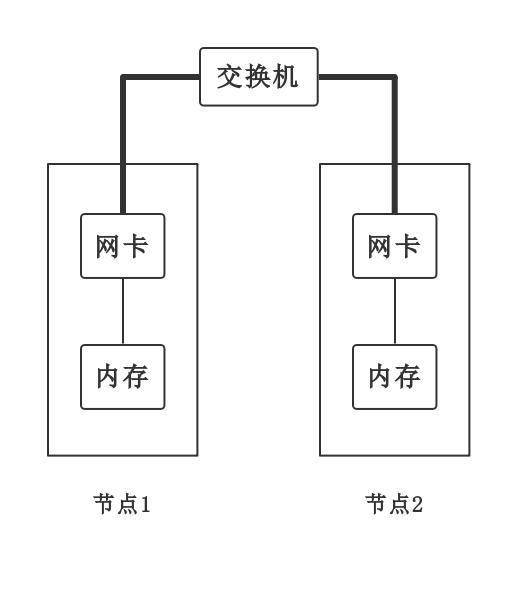
\includegraphics[width = 10cm]{topology.jpeg}
  \caption{两节点通信拓扑结构图}
  \label{fig:topology}
\end{figure}

根据上一节的分析,若算法可以在稀疏矩阵格式下直接进行按位加法操作,其计算量是非常小的,Allreduce的瓶颈主要在各设备之间的通信延迟。由于计算量较小,并不需要计算性能很高的CPU或GPU设备,所以在接下来本文设计的算法中可以使用智能网卡。智能网卡的引入可以避免每轮传输中机器内部从内存到网卡的两次传输延迟,即每轮通信只发生在网卡与交换机之间(图\ref{fig:topology}中的加粗部分),主机端内存并不参与其中。并且由于稀疏矩阵加法的计算量非常小,即使智能网卡上的CPU性能没有主机端的CPU性能高,也并不会导致产生过多的额外计算时间。

\section{算法设计}
\subsection{稀疏矩阵的存储格式}
\label{subsec:sparse-format}
%可以考虑在第二章介绍一下稀疏矩阵存储格式
%在前文中(引用)我们介绍过多种稀疏矩阵的存储格式,但它们都不太适合稀疏的神经网络梯度矩阵的通信。
在大多数深度学习框架中,神经网络的每一层参数都存储在连续的内存中,在进行分布式训练的反向传播时,它们会计算出网络中每一层参数的梯度,等整个网络的梯度都计算完成后,将每层的梯度拼接在一起,形成一个完整且连续的梯度矩阵。与其说是梯度矩阵,不如说成是梯度向量会更合适,因为它们在内存中是连续的。

经典的稀疏矩阵存储格式,如CSC,CSR等,它们能高效地存储二维矩阵,但对于一维的向量而言,反而会带来不必要的存储开销。所以本文选择了更适用于一维稀疏向量且能够支持稀疏格式下的直接加法的存储格式。

可以将这种存储格式抽象为:
[($index_0$, $val_0$), ($index_1$, $val_1$), ($index_2$, $val_2$), $\cdots$, ($index_{n-1}$, $val_{n-1}$)]。

其中,$index_i$表示表示第i个非零元在矩阵按行展开后的位置,也就是相对于矩阵在内存中的起始地址而言,第i个非零元在内存中的相对位置;而$val_i$则表示第i个非零元的数值。

\begin{figure}[ht] % use float package if you want it here
  \centering
  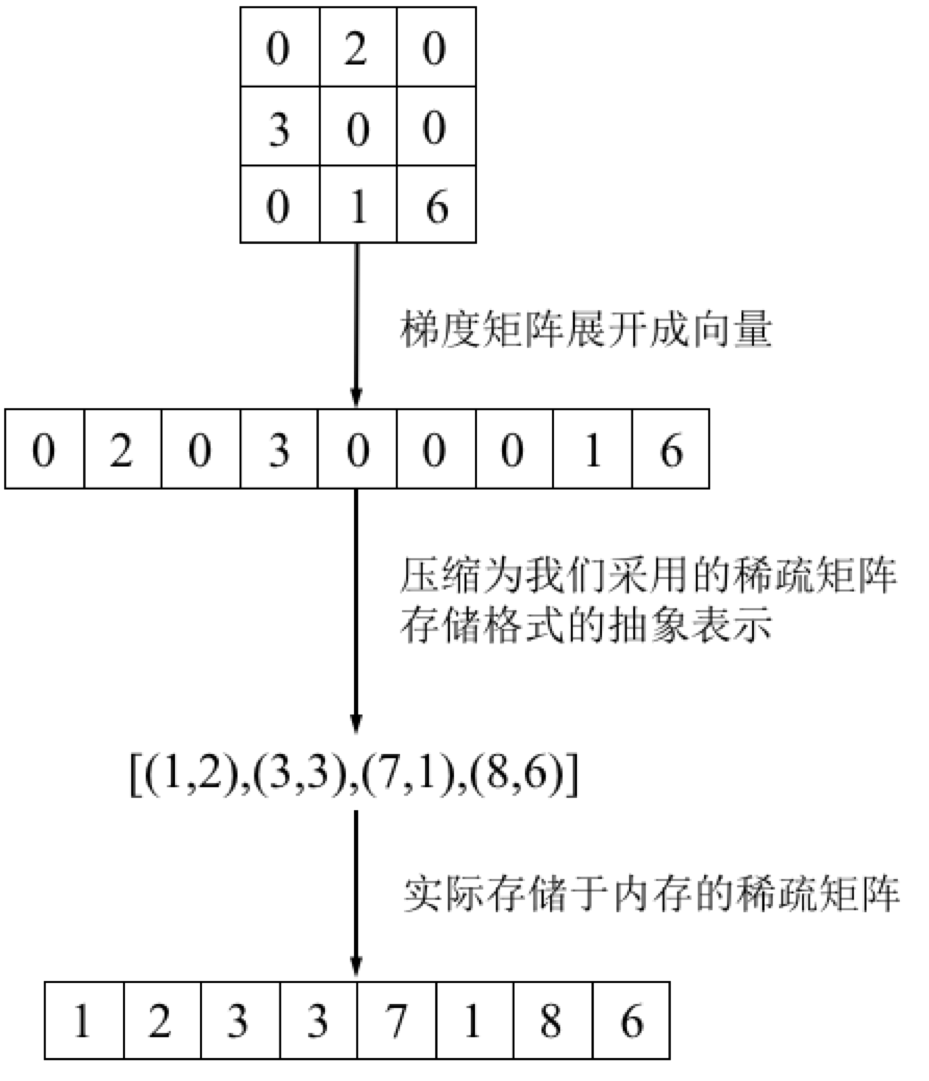
\includegraphics[width = 11cm]{sparse-format.png}
  \caption{稀疏矩阵的存储格式}
  \label{fig:sparse-format}
\end{figure}

在图\ref{fig:sparse-format}中可以更形象、清楚地看出本文所采用的存储格式的实际含义。在实际应用中,梯度矩阵中存储的都是浮点数,但是为了方便,在本文中将以整数的形式表示。

\subsection{稀疏矩阵的加法}
本文设计的稀疏格式下的加法算法的思想类似于归并排序,不过是以index为关键字而不是以val为关键字。算法伪代码如下,输入为两个稀疏矩阵和它们的非零元个数:
\makeatletter
\def\BState{\State\hskip-\ALG@thistlm}
\makeatother
\begin{algorithm}
\begin{algorithmic}[1]
\Procedure{SPARSE-ADDITION}{$src_0, src_1, num_0, num_1$}
\State $index_0 \gets 0$
\State $index_1 \gets 1$
\For{$i \gets 0 $ to $num_0 + num_1 - 1$}
\If{$index_1 >= num_1$ \textbf{or} $src_0[index_0].index < src_1[index_1].index$}
\State $dst[i].index \gets src_0[index_0].index$
\State $dst[i].value \gets src_0[index_0].value$
\State $index_0 \gets index_0 + 1$
\ElsIf{$index_0 >= num_0$ \textbf{or} $src_0[index_0].index > src_1[index_1].index$}
\State $dst[i].index \gets src_1[index_1].index$
\State $dst[i].value \gets src_1[index_1].value$
\State $index_1 \gets index_1 + 1$
\ElsIf{$src_0[index_0].index = src_1[index_1].index$}
\State $dst[i].index \gets src_0[index_0].index$
\State $dst[i].value \gets src_0[index_0].value + src_1[index_1].value$
\State $index_0 \gets index_0 + 1$
\State $index_1 \gets index_1 + 1$

\EndIf
\EndFor
\State \Return $dst$
\EndProcedure
\end{algorithmic}
\end{algorithm}


如图\ref{fig:sparse-addition}为稀疏矩阵加法的示意图。

\begin{figure}[ht] % use float package if you want it here
  \centering
  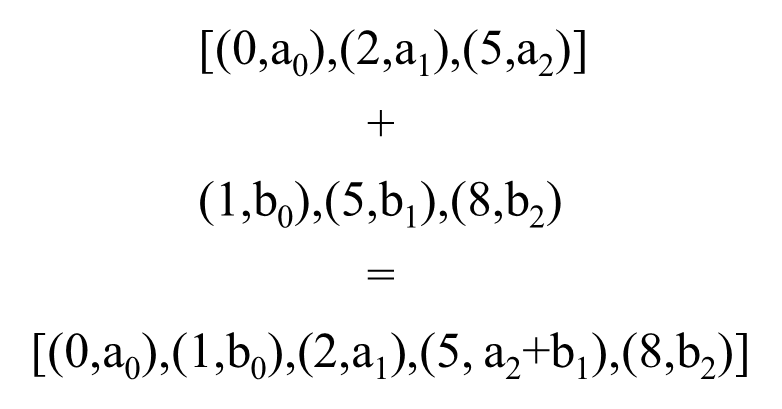
\includegraphics[width = 11cm]{sparse-addition.png}
  \caption{稀疏矩阵的加法}
  \label{fig:sparse-addition}
\end{figure}

前文提到,这个算法类似于归并排序,且是以index作为关键字。这实际上对应着本文设计的算法需要满足的一条重要的性质:输入的两个稀疏矩阵中的index必须是有序的。这就类似于在归并排序中,需要进行归并的两个数组中的元素必须是有序的一样。只有输入的两个稀疏矩阵中的index有序,才能够保证算法的正确性;换句话说,如果index无序的话,就无法正确的将两个index相同的val正确地进行合并。

幸运的是,根据算法流程,只要输入的两个稀疏矩阵中的index是有序的,输出的稀疏矩阵中的index也将会是有序的。这也就意味着,只需要确保所有梯度矩阵在压缩时可以按照index的顺序进行压缩,之后所有轮次中的稀疏矩阵相加的正确性就是有保证的,这可以使用数学归纳法进行证明。

有了稀疏矩阵的加法,就可以只在Allreduce算法的最开始进行一次梯度矩阵的压缩,且只在Allreduce算法结束前进行一次稀疏矩阵的解压缩,在Allreduce算法的每一轮中不需要再进行压缩或解压缩,直接进行稀疏矩阵的加法即可,这大大缩短了Allreduce算法的执行时间。

同时,稀疏矩阵的加法避免了普通按位Reduce操作中,由于梯度矩阵过于稀疏而导致的大量冗余的零元加法。

\subsection{Allreduce算法选择}
在本文的算法中,Allreduce的每一轮通信都是传输一个稀疏矩阵,相对于传统深度学习分布式训练的多机通信而言,本文的算法通信量并不大。

随着通信量的减少,通信部分的瓶颈不在网络带宽,而在网络延迟。拥有“总通信量少”的特点的环形Allreduce算法将不再具有优势,同时,环形算法的“轮数多”的特点将会使得网络延迟更为严重。大多数深度学习框架所采用的环形Allreduce算法对于本文而言并不合适。

本文选择使用蝶形算法,在进程数为n时,蝶形算法只需要用$\lceil log_2(n) \rceil$轮就可以完成Allreduce算法。虽然蝶形算法的总通信量较大,但由于通信的是比较小的稀疏矩阵,所以这并不会为Allreduce算法带来较多的额外通信时间。

\subsection{使用智能网卡降低设备传输延迟}
综合前文所述,现在可以把本文所设计的算法流程概括如下(为方便起见,只考虑进程数为2的正整数次幂的情况。算法轮数从0开始计数,进程数从0开始计数,每台机器只启动一个进程执行分布式训练):
\begin{itemize}
  \item [1)]
  进程将梯度矩阵输入进随机选择算法,选出梯度矩阵中第$\frac{size}{1000}$大的浮点数作为阈值,其中,size为梯度矩阵中浮点数的个数。
  \item [2)] 
  通过随机选择法得到的阈值,筛选出稠密度为$\frac{1}{1000}$的矩阵,并将其压缩成第\ref{subsec:sparse-format}节中描述的稀疏矩阵格式,将得到的稀疏矩阵设置为本地稀疏矩阵。
  \item [3)]
  在算法的第i轮,第x台机器与第x xor $2^i$台机器进行通信,这两台机器别将自己的本地稀疏矩阵发送给对方,并从对方接收对方发送来的的稀疏矩阵。
  \item [4)]
  将自己的本地稀疏矩阵与接收的对方的稀疏矩阵进行稀疏矩阵加法,将加法得到的矩阵再次设置为本地稀疏矩阵。
  \item [5)]
  重复过程3)$\sim$4),直到$log_2(n)$轮的蝶形算法完成。
  \item [6)]
  将本地稀疏矩阵解压缩为梯度矩阵,用于更新模型参数。
\end{itemize}

若要更细粒度地、从设备的角度分析Allreduce算法的通信过程,可以将过程3)扩充如下:
\begin{itemize}
  \item [3.1)]
  存储于每一台机器内存中的本地稀疏矩阵被传输到机器的网卡内。
  \item [3.2)]
  第x台机器的网卡与第x xor $2^i$台机器的网卡之间通过交换机等设备进行通信,这两台机器的网卡别将自己的本地稀疏矩阵发送给对方网卡,并从对方接收对方发送来的的稀疏矩阵。
  \item [3.3)]
  每台机器将网卡接收到的稀疏矩阵发送至机器内的内存。
\end{itemize}

根据前文分析,由于本文所采用算法的通信量较少,通信的瓶颈在延迟,降低传输延迟就能够有效缩短算法执行时间。为了能够降低通信延迟,本文已经使用了通信轮数更少的Allreduce算法,若要想进一步降低通信延迟,还可以减少参与一轮通信的设备数。

若使用标准网卡进行通信,如3.1)$\sim$3.3)所描述的那样,每轮通信所要经过的设备是内存$\rightarrow$网卡$\rightarrow$交换机$\rightarrow$网卡$\rightarrow$内存。若使用具有计算功能的智能网卡,就可以将稀疏矩阵加法放在网卡上进行计算,主机端中央处理器不再需要进行稀疏矩阵的加法,每轮通信也就不再需要将信息发送至主机端内存。这样可以将参与每轮通信的设备缩减至网卡$\rightarrow$交换机$\rightarrow$网卡。

尽管智能网卡上的中央处理器的计算性能不如主机端的中央处理器,但是用于计算稀疏矩阵的加法还是绰绰有余的。稀疏矩阵加法的计算量并不大,它并不是一个计算密集型任务,在接下来的实验中我们也将看到,稀疏矩阵加法是各项操作中(包括压缩、解压缩、第k大梯度选择以及稀疏矩阵通信)耗时最短的。所以使用性能较差的网卡上的中央处理器进行稀疏矩阵加法也并不会在计算上引入过多的额外时间,反而能够通过不将稀疏矩阵与主机端的内存进行通信而达到降低传输延迟的效果。

不过相比于计算量较少的稀疏矩阵加法,对于压缩和解压缩这种计算量较大的操作,还是更适合放在主机端中央处理器来进行计算。也就是说,若使用智能网卡,则在Allreduce算法的最开始,由主机端中央处理器将梯度矩阵压缩成稀疏矩阵,并将其发送至智能网卡。之后Allreduce的每轮通信与稀疏矩阵加法都只在各个智能网卡之间进行,不经过主机端中央处理器和内存。等Allreduce算法的所有轮通信都执行完之后,智能网卡再将稀疏矩阵发送至主机端内存,并由主机端中央处理器将其解压缩至梯度矩阵。

\subsection{第k大梯度选择的优化}
\label{subsec:topKOptimize}
前文中我们介绍过随机选择算法,该算法可以在期望$\Theta(n)$的时间内找到n个元素的数组中第k大的数值。

虽然随机选择算法的计算复杂度较低,且算法主体的访存是连续的,对cashe比较友好,但是算法常数仍然比较大,执行速度较慢。经分析,其原因主要是在随机选择算法的RANDOMIZED--PARTITION函数中,有大量的条件判断语句将一个数组中的元素与固定的关键字进行比较。由于关键字是从所有数值中随机选择出来的,所以任何一个数值与关键字的大小关系是随机的,这就导致了中央处理器的分支预测技术预测出的分支结果的正确率非常低(平均只有50\%)。又由于分支预测失败后的开销较大,所以随机选择算法的常数比较大。遗憾的是,由于随机选择算法本身设计,这种分支预测的失败是无法避免的。

同时,随机选择算法的RANDOMIZED--PARTITION部分几乎无法使用多线程等方法来通过并行计算取得加速效果,所以随机选择算法本身几乎无法优化。

既然随机选择算法难以优化,且随机选择算法的执行时间又与输入算法的数据量有关,那么若想要减少随机选择算法的执行时间,一个很直观的想法就是减少输入随机选择算法的数据量。若减少了输入随机选择算法的数据量,为了保证算法的正确性,也就是随机选择算法能够正确的选择出原梯度矩阵中所有数值的第$\frac{size}{1000}$大的数值,而不是输入随机选择算法中的第$\frac{n}{1000}$大的数值\footnote{size为原梯度矩阵中浮点数的个数,n为输入随机选择算法的浮点数的个数},也就需要保证,原梯度矩阵中的前$\frac{size}{1000}$大的所有数值,都要被输入随机选择算法。

为了找出原梯度矩阵中的前$\frac{size}{1000}$大的所有数值,就需要用一个数值作为阈值去筛选原梯度矩阵,这个阈值必须要比前$\frac{size}{1000}$大的数值小,但是由于之后要将筛选出的数值输入随机选择算法,所以为了随机选择算法执行时间更短,就需要让被筛选出的数值尽量少,或者说,需要让阈值在比前$\frac{size}{1000}$大的数值小的同时尽量大。为了得到这样的一个阈值,本文采用的方法就是先采样,再调用随机选择算法。

本文设计的第k大梯度选择的算法流程如下:
\begin{itemize}
  \item [1)]
  设置k大值比例topK\_ratio为0.5\%。
  \item [2)]
  对原梯度矩阵进行采样,采样共$\frac{size}{100}$个数值,将它们输入至随机选择算法,选择出它们中的第$\frac{size}{100}\times sample\_ratio$大的数值作为阈值。
  \item [3)]
  使用阈值对原梯度矩阵进行筛选,将大于阈值的梯度筛选出来。
  \item [4)]
  将被筛选出的梯度的数量与$\frac{size}{1000}$进行比较,若被筛选出的梯度的数量小于$\frac{size}{1000}$,则说明选择的阈值大于原梯度矩阵中第$\frac{size}{1000}$大的梯度,需要重新选择阈值。为了使阈值更大,就将k大值比例变为原来的两倍,即$topK\_ratio = topK\_ratio \times 2$,并跳转到2)继续执行;直到被筛选出的梯度的数量大于或等于$\frac{size}{1000}$。
  \item [5)]
  将被筛选出的梯度输入随机选择算法,选出它们中的第$\frac{size}{1000}$大的数值。
\end{itemize}

算法中的采样的梯度对选出来的阈值有很大影响。若采样的梯度整体偏大,则选出的阈值也会比较大,反之亦然。在理想情况下,原梯度矩阵分布均匀,采样的梯度也就可以代表原梯度矩阵,所选出的阈值也会比较合适,即在比前$\frac{size}{1000}$大的梯度小的同时尽量大。但是实际上,在神经网络反向传播中,梯度的分布并不会非常均匀。为了使得采样尽量均匀,我们会在梯度矩阵中选择多处位置,每一处采样连续的一段梯度,然后将各处的采样拼接到一起,作为最终的采样结果输入值随机选择算法。

但是,即使采用了这种尽量均匀的采样方式,采样得到的梯度分布也依然不会和原梯度矩阵的分布是一样的。若根据采样梯度选出的阈值比原梯度矩阵中第$\frac{size}{1000}$大的梯度还要大的话,之前所选出来的阈值就没有任何意义,随机选择算法所消耗的时间也将白白浪费。所以,提高选出可用的阈值的概率,我们将随机选择算法要选择的k大值的比例由0.1\%提高到0.5\%。这样一来,即使采样并不够均匀,但是采样的梯度中第$\frac{sample\_size}{200}$大的梯度\footnote{sample\_size为采样的梯度数量,即$\frac{size}{100}$}很大概率上还是会小于原梯度矩阵中第$\frac{size}{1000}$的梯度。

即使有了选取多段采样以及提高k大值的比例这两项措施,随机选择算法选出的阈值仍然可能不满足小于原梯度矩阵中第$\frac{size}{1000}$大梯度的要求。这时,算法会再次提高k大值的比例,重新采样并调用随机选择算法选取阈值,直到选取出满足条件的阈值为止。

这个算法流程虽然看似步骤繁多,但这并不会使得算法执行时间较长,因为算法的每一步设计的数据量比较小。比如采样并输入进随机选择算法的梯度只有原梯度矩阵的1\%,并且在平均情况下,通过阈值筛选出来并输入随机选择法算法的梯度只有原梯度矩阵的0.5\%。而在前文中提到了随机选择算法的时间复杂度为$\Theta(n)$,那么相比于将原梯度矩阵全部输入进随机选择算法,通过对梯度矩阵的处理,随机选择算法的执行时间将只有原来的1.5\%左右。

算法中最耗时的部分是使用阈值筛选原梯度矩阵,这一步需要遍历梯度矩阵中所有梯度。不过,在平均情况下,算法选出的阈值会大于梯度矩阵中99.5\%的梯度,所以中央处理器的分支预测会有极高的准确率,代码执行速度也会非常快。经过测试,在单线程下,与使用原梯度矩阵直接调用随机选择算法相比,经过本文优化后的第k大梯度选择过程的速度提高了13.3倍。

同时,最耗时的筛选过程可以使用多线程进行并行计算,这样就能进一步缩短算法执行时间。

\subsection{算法总述}
本文从四个方面对稀疏矩阵的Allreduce过程进行优化,如图\ref{fig:summary}所示。

\begin{figure}[ht] % use float package if you want it here
  \centering
  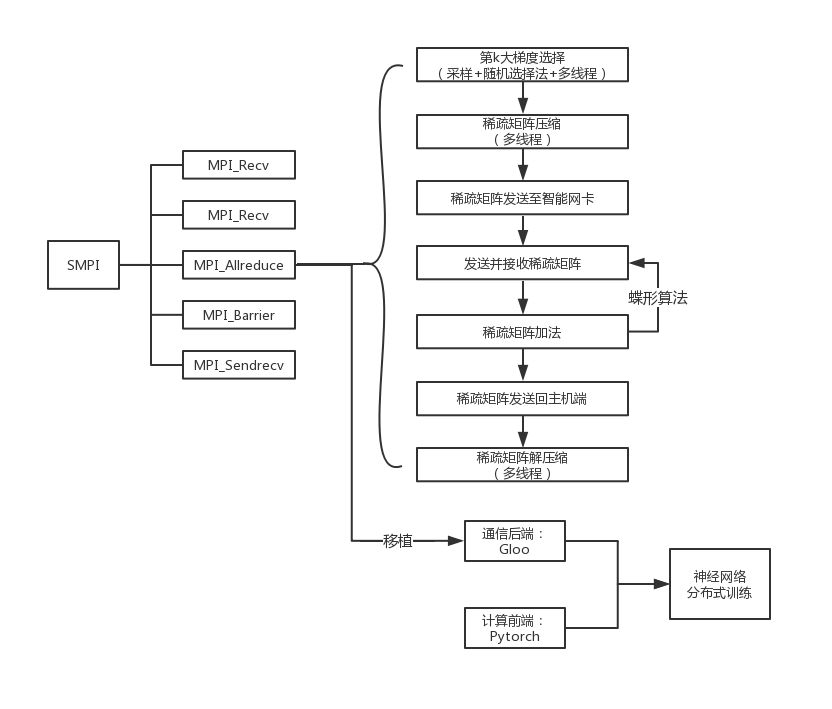
\includegraphics[width = 15cm]{summary.png}
  \caption{算法总述}
  \label{fig:summary}
\end{figure}

在本文提出的优化算法中,首先使用基于采样的方法,通过多次调用随机选择算法来对第k大梯度的选择过程进行加速。根据选择出的阈值,再将梯度矩阵压缩为稀疏矩阵。之后将稀疏矩阵发送至智能网卡,并在智能网卡之间执行蝶形算法。蝶形算法的每一轮,智能网卡会先发送并接受稀疏矩阵,之后在智能网卡上直接进行稀疏矩阵的加法,不需要压缩与解压缩操作。蝶形算法只发生在智能网卡之间,主机端并不参与其中。蝶形算法结束后,智能网卡将稀疏矩阵再发送至主机端,由主机进行稀疏矩阵的解压缩。对于第k大梯度选择与稀疏矩阵的压缩和解压缩过程,本文都使用了多线程并行计算。